\StartPlate{V09}{Where the original dyadic quotient runs out of room}{The rank-eight case is the first equality, not a low-rank surplus.}
\begin{center}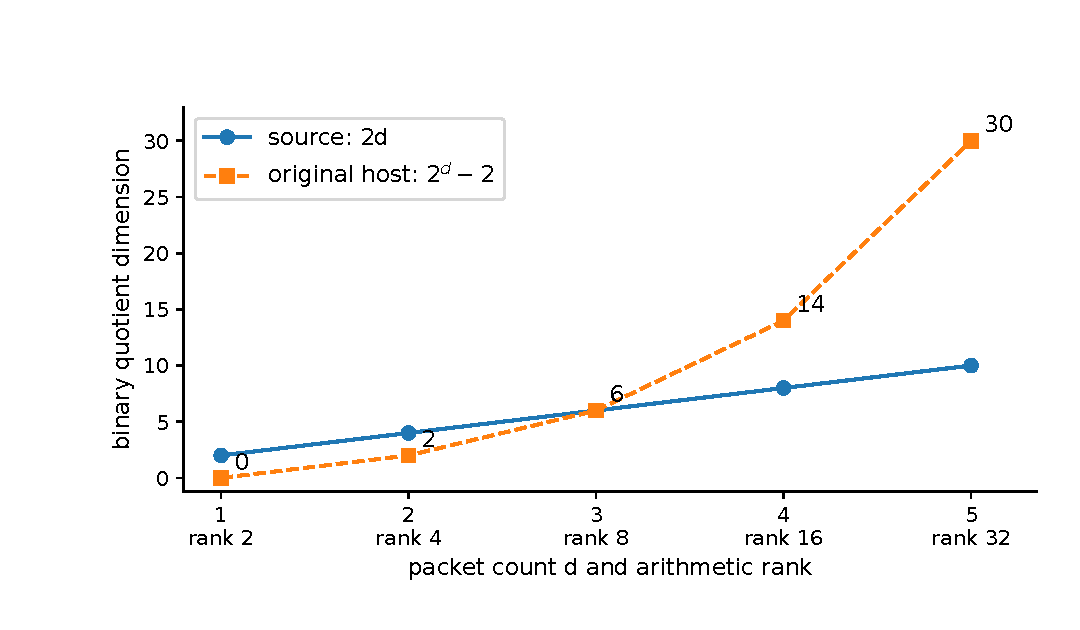
\includegraphics[width=\linewidth]{figures/V09.pdf}\end{center}
For $d$ source planes, the binary source quotient has dimension $2d$. In the full dyadic profile the specified original maximal-type quotient has dimension $D=2^d-2$. The first five values are shown without normalizing away their difference.
\[
\begin{array}{c|ccccc}
d&1&2&3&4&5\\
2d&2&4&6&8&10\\
2^d-2&0&2&6&14&30
\end{array}
\]
Ranks two and four are too small in that original quotient. Rank eight has exactly six dimensions for six required dimensions. Only from rank sixteen is there a strict surplus in this family.

The later low-rank repair uses a larger actual assembly carrier and recovers the same representation. It does not change the first two numbers in this table. At equality, a fixed native quadratic refinement can still obstruct attachment. With spare dimension, the free quadratic embedding problem is easier, but prescribed actions, lifts, and transports remain separate constraints.
\vfill\PlateSource{Exact capacity formula}{Part I, Section 9; Part III, Section 24.2}{21}
